\documentclass[11pt]{article}
\usepackage[margin=1in]{geometry}
\usepackage[T1]{fontenc}
\usepackage{lmodern}
\usepackage{amssymb}
\usepackage{booktabs}
\usepackage{tabularx}
\usepackage{graphicx}
\usepackage{subcaption}
\usepackage{enumitem}
\usepackage[hidelinks]{hyperref}
\setlist{itemsep=2pt,topsep=4pt}
\newcolumntype{Y}{>{\raggedright\arraybackslash}X}

\title{Can an AI Find Its Own Mistakes?\\[4pt]
\large Self-Evolving Metamorphic Testing of Language and Vision Models}
\author{CS6223 Course Project}
\date{2026}

\begin{document}
\maketitle

% ---------------------------------------------------------------
\section{Summary}

We built a closed loop in which an AI model \textbf{tests itself}. The model writes small Python programs that
change a test question in a way that should keep the correct answer the same (shuffle the options, reword the
question, add noise to the picture, \ldots). Then the same model answers both the original and the changed
question. If the answer changes, we found a failure. Programs that find real failures get more tests; programs
that make unfair changes are repaired or retired. No human is in the loop.

We tested Qwen3 1.7B / 8B / 32B on MMLU (text) and Qwen3-VL 2B / 8B / 32B on ScienceQA (images).

Main findings:
\begin{enumerate}
  \item \textbf{The hard part is not finding failures, it is knowing if they are real.} A changed question can
        quietly change the answer. When the model judged its own tests, about 4 in 10 ``failures'' it accepted
        were really broken tests.
  \item \textbf{Hiding the answer from the programs helps a lot.} When the programs could see the correct answer,
        81\% of the failures they found were broken. With the answer hidden, 80--89\% were real (1.7B).
  \item \textbf{A self-evolving loop ``games'' the judge if allowed.} Our ``Bold'' version found 2--3$\times$ more
        failures, but most of the extra ones were tricks such as ``Which is \textbf{NOT NOT} \ldots?''. Simple
        code rules (``Bold + rules'') removed the tricks.
  \item \textbf{Final result (Bold + rules):} on text, slightly more real failures than hand-written programs
        (8B: 59 vs 49, 32B: 39 vs 33, 1.7B: 100 vs 99). On images, clearly more on the strongest model
        (32B: $\sim$37 vs 16), but fewer on the smaller ones, because many changed pictures were destroyed and
        the grader did not notice.
\end{enumerate}

% ---------------------------------------------------------------
\section{The problem in one example}

Question (MMLU, logical fallacies): \emph{``The complex proposition fallacy involves \ldots''}

\begin{center}
\begin{tabularx}{\linewidth}{lYl}
\toprule
 & Options & Qwen3-32B says \\
\midrule
Original & \textbf{A = ``including more than one claim \ldots''} (correct), B, C, D & \textbf{A} \checkmark \\
Options shuffled & the same correct text is now option \textbf{C} & \textbf{A} $\times$ \\
\bottomrule
\end{tabularx}
\end{center}

The answer should simply move from A to C. The model kept ``A''. This is a real failure (``metamorphic
violation'').

But not every change is fair:

\begin{center}
\begin{tabularx}{0.9\linewidth}{Yl}
\toprule
Change & Fair? \\
\midrule
Shuffle the options & Fair: answer moves in a known way \\
``Which is \textbf{NOT NOT} the difference between \ldots'' & Trick: technically the same, but no person writes this \\
Image so noisy the labels can't be read & Broken: the information needed to answer is gone \\
\bottomrule
\end{tabularx}
\end{center}

So every found failure needs a \textbf{judge}: ``is the right answer still the same?''

% ---------------------------------------------------------------
\section{Method}

\paragraph{Programs.} Each change is a Python function \texttt{mutate(seed, rng)} plus a
\texttt{check(seed, mutated)} that rejects bad output. We start from 7 hand-written text programs (paraphrase,
typo noise, option shuffle, \ldots) and 9 image programs (blur, noise, JPEG, brightness, option shuffle, \ldots).
The model then writes new programs and ``stronger variants'' of good ones. Programs run in a sandbox with a time
limit.

\paragraph{Answer hidden.} Programs never see which option is correct. They must be fair to \emph{whichever}
option is correct.

\paragraph{Judging.} Each changed question passes:
\begin{enumerate}
  \item \emph{Fixed code checks:} options must be a true shuffle, numbers must not disappear, and (Bold + rules
        only) no added negation word, the question must stay in one piece, options must not become much longer.
  \item \emph{AI judge} (GLM, through an API): ``Is the correct answer still the same?''
\end{enumerate}

\paragraph{Feedback.} Programs that find accepted failures get more tests (a bandit score). Programs whose output
is rejected get a repair attempt, and the repair is tested before it is accepted. Programs that find nothing for a
long time are retired. (Bold + rules only) One program family can get at most 25\% of the tests, so one trick
can't take over.

\paragraph{Grading (evaluation only).} After each run, a different AI (DeepSeek) grades every failure. We then
hand-checked samples ourselves (an AI assistant acted as a ``pseudo-human'' labeler; 210 text and 40 image cases).

\paragraph{Versions we compare.}

\begin{center}
\begin{tabularx}{\linewidth}{lY}
\toprule
Name & What changed \\
\midrule
Hand-written & Only the hand-written programs, no evolution (baseline) \\
Self-judged & Evolving programs, the model judges its own tests \\
Outside judge & Another AI (GLM) judges, answer hidden from programs \\
Bold & Push for stronger changes, retire useless programs, code checks, tested repairs \\
Bold + rules & Bold, plus rules against tricks (added negation, broken-up question, padded options) and a 25\% cap.
  \textbf{Our final version.} \\
\bottomrule
\end{tabularx}
\end{center}

\paragraph{Setup.} 5,000 model calls per run (judge calls not counted), 3 runs (seeds) per setting, results are
mean $\pm$ std. Main metric: \textbf{number of different questions with a failure} that the grader accepts
(``real'').

% ---------------------------------------------------------------
\section{Results: text (MMLU)}

Table~\ref{tab:text} shows the number of different questions with a real failure (DeepSeek-graded).
``Bold, tricks removed'' leaves out double negations and broken-up questions.

\begin{table}[h]
\centering
\caption{Text: different questions with a real failure.}
\label{tab:text}
\begin{tabular}{lrrrrrr}
\toprule
Model & Hand-written & Self-judged & Outside judge & Bold & \shortstack{Bold,\\tricks removed} & \textbf{Bold + rules} \\
\midrule
1.7B & 99 & 109 & 55 & 170 & 169 & \textbf{100} \\
8B   & 49 & 40  & 60 & 135 & 57  & \textbf{59} \\
32B  & 33 & 26  & 28 & 80  & 31  & \textbf{39} \\
\bottomrule
\end{tabular}
\end{table}

\begin{table}[h]
\centering
\caption{Text: share of found failures that are real.}
\label{tab:textshare}
\begin{tabular}{lrrrrr}
\toprule
Model & Hand-written & Self-judged & Outside judge & Bold & Bold + rules \\
\midrule
1.7B & 76\% & 56\% & 80\% & 81\% & \textbf{89\%} \\
8B   & 80\% & 15\% & 48\% & 77\% & 42\% \\
32B  & 79\% & 30\% & 44\% & 72\% & 62\% \\
\bottomrule
\end{tabular}
\end{table}

What this means:
\begin{itemize}
  \item \textbf{Self-judged is poor:} for 8B only 15\% of its failures are real. The model can't judge its own
        tests.
  \item \textbf{Bold looked great but was gaming the judge.} For 8B and 32B almost all of its gain came from
        ``NOT NOT'' and broken-up questions; with these removed, Bold is back near Hand-written (57 vs 49, 31 vs 33).
  \item \textbf{Bold + rules is honest:} it gives the same number with or without trick removal, and it is a little
        above Hand-written on 8B and 32B. The spread between runs is large (8B: 59 $\pm$ 40), so this is a small
        gain, not a clear win.
  \item Bold + rules on 8B has many false alarms (42\% real) in all three runs; one run alone produced 413 of the
        597 flagged cases.
\end{itemize}

Hand labels (text) confirm the judges' behavior: of 102 changes the self-judge accepted, 38 were broken; of 54
changes GLM accepted in Bold, 32 were tricks; DeepSeek accepted no truly broken text change but did accept tricks.

Programs could see the answer (one 1.7B run of Outside judge): 409 failures, only 19\% real.
\textbf{Hiding the answer is essential.}

% ---------------------------------------------------------------
\section{Results: images (ScienceQA)}

\begin{table}[h]
\centering
\caption{Images: different questions with a failure, as graded by DeepSeek, and corrected by hand-check.}
\label{tab:img}
\begin{tabular}{lrrrr}
\toprule
Model & Hand-written & Self-judged & \shortstack{Bold + rules\\(DeepSeek)} & \shortstack{Bold + rules\\(hand-corrected)} \\
\midrule
VL-2B  & 40 & 27 & 39  & $\sim$20 \\
VL-8B  & 29 & 46 & 101 & $\sim$13 \\
VL-32B & 16 & 12 & 50  & $\sim$37 \\
\bottomrule
\end{tabular}
\end{table}

\begin{table}[h]
\centering
\caption{Hand-check of 40 DeepSeek-accepted image failures (blind, mixed).}
\label{tab:imgcheck}
\begin{tabular}{lrrr}
\toprule
 & fair & trick & broken \\
\midrule
Hand-written (20)        & 20 & 0 & 0 \\
Bold + rules, VL-2B (4)  & 2  & 2 & 0 \\
Bold + rules, VL-8B (8)  & 1  & 1 & 6 \\
Bold + rules, VL-32B (8) & 6  & 0 & 2 \\
\bottomrule
\end{tabular}
\end{table}

Figure~\ref{fig:examples} shows one fair and two broken examples.

\begin{figure}[h]
\centering
\begin{subfigure}{\linewidth}\centering
  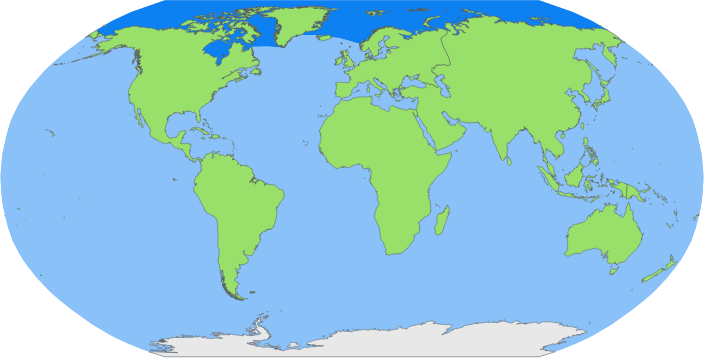
\includegraphics[height=3.2cm]{figures/fair_orig.png}\hspace{6pt}
  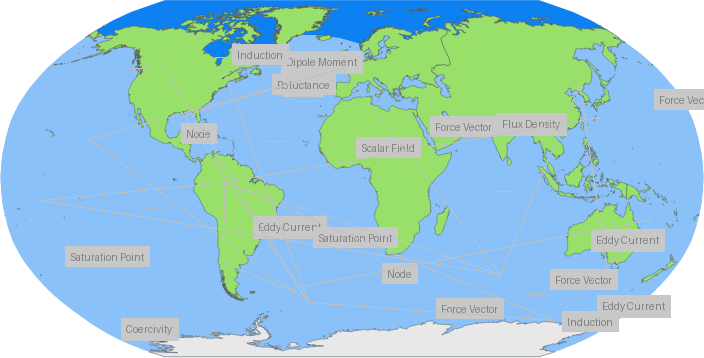
\includegraphics[height=3.2cm]{figures/fair_new.png}
  \caption{\textbf{Fair:} world map with random science words pasted on it; the highlighted ocean is still clear.
           VL-32B answered wrong.}
\end{subfigure}\\[8pt]
\begin{subfigure}{0.48\linewidth}\centering
  
\includegraphics[height=2.8cm]{figures/broken_orig.png}\hspace{4pt}
  
\includegraphics[height=2.8cm]{figures/broken_new.png}
  \caption{\textbf{Broken:} a wooden spatula with colors inverted, so it looks like blue plastic
           (``what material is it?'').}
\end{subfigure}\hfill
\begin{subfigure}{0.48\linewidth}\centering
  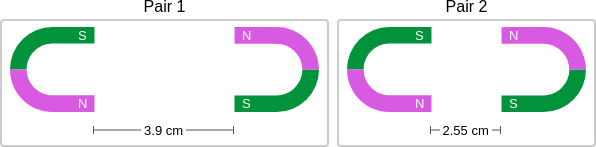
\includegraphics[height=2.8cm]{figures/broken2_orig.png}\hspace{4pt}
  
\includegraphics[height=2.8cm]{figures/broken2_new.png}
  \caption{\textbf{Broken:} magnets pixelated until the N/S labels and distances can't be read.}
\end{subfigure}
\caption{Image changes made by Bold + rules (left: original, right: changed).}
\label{fig:examples}
\end{figure}

What this means:
\begin{itemize}
  \item The hand-written image programs are mild and always fair, but find few failures.
  \item Bold + rules learned to make \textbf{stronger} image changes. On VL-32B many are fair and it finds about
        twice as many real failures as Hand-written. On VL-8B it went too far: most images were destroyed.
  \item \textbf{The image grader is too lenient:} DeepSeek often says ``still answerable'' for pictures a person
        can't read. Without the hand-check, we would have reported a 3$\times$ gain on VL-8B that is not real.
\end{itemize}

% ---------------------------------------------------------------
\section{Limitations}

\begin{itemize}
  \item Hand labels were made by an AI assistant acting as a careful human labeler, on samples (210 text, 40 image);
        the image correction uses only 4--8 cases per model, so those numbers are rough.
  \item 3 runs per setting; the spread between runs is large.
  \item One dataset per task, one model family (Qwen3).
  \item We could not stop image changes that destroy information; a check such as ``small text must still be
        readable'' is the obvious next step.
\end{itemize}

% ---------------------------------------------------------------
\section{Conclusion}

A model can find its own failures, but \textbf{only if someone else checks the tests}. The model judging itself
gives many false alarms. A self-evolving loop is very good at finding ways to fool its judge, so the judge must be
backed by simple code rules, and the results must be spot-checked by hand. With these in place, the self-evolving
loop gives a modest gain on text and a clear gain on the strongest image model. Its main weakness is that it
pushes image changes until they destroy the picture.

\end{document}
